\documentclass[conference]{IEEEtran}
\IEEEoverridecommandlockouts
% The preceding line is only needed to identify funding in the first footnote. If that is unneeded, please comment it out.
\usepackage{cite}
\usepackage{amsmath,amssymb,amsfonts}
\usepackage{algorithmic}
\usepackage{graphicx}
\usepackage{textcomp}
\usepackage{xcolor}
\usepackage{booktabs}
\usepackage{microtype}
\usepackage{hyperref}

\def\BibTeX{{\rm B\kern-.05em{\sc i\kern-.025em b}\kern-.08em
    T\kern-.1667em\lower.7ex\hbox{E}\kern-.125emX}}

\begin{document}

\title{AI-Driven Air Quality Forecasting and Multi-Pollutant Health Risk Alert System for Indian Metropolitan Cities\\
\thanks{This research was conducted in the Department of Computer Science \& Engineering, C.V. Raman Global University (CGU), Bhubaneswar, Odisha, India, under the faculty supervision of Prof. Soumya Sahoo.}
}

\author{
\IEEEauthorblockN{Satyaprakash Rout}
\IEEEauthorblockA{\textit{Dept. of Computer Science \& Engg.} \\
\textit{C.V. Raman Global University (CGU)}\\
Bhubaneswar, Odisha, India \\
satyaprakashrout435@gmail.com}
\and
\IEEEauthorblockN{Likuna Swain}
\IEEEauthorblockA{\textit{Dept. of Computer Science \& Engg.} \\
\textit{C.V. Raman Global University (CGU)}\\
Bhubaneswar, Odisha, India \\
likunaswain2@gmail.com}
\and
\IEEEauthorblockN{Ch Saipriya Patra}
\IEEEauthorblockA{\textit{Dept. of Computer Science \& Engg.} \\
\textit{C.V. Raman Global University (CGU)}\\
Bhubaneswar, Odisha, India \\
patrachsaipriya@gmail.com}
\and
\IEEEauthorblockN{Arpeet Barik}
\IEEEauthorblockA{\textit{Dept. of Computer Science \& Engg.} \\
\textit{C.V. Raman Global University (CGU)}\\
Bhubaneswar, Odisha, India \\
arpeetbarik954@gmail.com}
\and
\IEEEauthorblockN{Prof. Soumya Sahoo}
\IEEEauthorblockA{\textit{Faculty Supervisor \& Guide} \\
\textit{Dept. of Computer Science \& Engg.} \\
\textit{C.V. Raman Global University (CGU)}\\
Bhubaneswar, Odisha, India}
}

\maketitle

\begin{abstract}
\bfseries Ambient air pollution across Indian metropolitan airsheds represents an acute environmental and public health crisis. Conventional National Air Quality Index (AQI) monitoring frameworks rely on retrospective sensor registries and heuristic single-pollutant maximum rules that systematically underestimate synergistic multi-pollutant toxicological risk. This paper presents VayuDrishti, an end-to-end artificial intelligence architecture for forward-looking 24-hour predictive AQI forecasting and clinically stratified public health alerting across primary Indian metropolitan airsheds (Delhi, Mumbai, Bengaluru, Hyderabad). The proposed methodology introduces a unified three-tier computational framework: (1) an automated Multimodal Imputation with Symmetrical Autoencoder (MI-MMA) pipeline that resolves telemetry dropouts via Multivariate Imputation by Chained Equations (MICE, $\text{RMSE} = 0.0061$) and compresses multi-pollutant manifolds into 36-dimensional bottleneck representations; (2) an Optuna-tuned Dual Stacking Ensemble (XGBoost, CatBoost, Random Forest, and non-negative Ridge meta-learner) augmented with ERA5 atmospheric boundary-layer parameters and episodic festival/crop-residue burning indicators, achieving test $R^2 = 0.9248$, $\text{RMSE} = 13.84$ AQI points, and a continuous regression accuracy of 91.42\%; and (3) an epidemiological Multi-Pollutant Health Risk Index (HRI) incorporating cohort-specific vulnerability multipliers (General: 1.0$\times$, Children/Elderly: 1.3$\times$, Pre-existing Respiratory: 1.6$\times$) yielding 24.9\% to 55.7\% clinical alert differentiation. Paired parametric Student's $t$-test ($t = -3.722, p = 0.0002$) and non-parametric Wilcoxon signed-rank test ($p = 3.003 \times 10^{-5}$) establish rigorous statistical superiority over classical regressors and deep recurrent sequence baselines. TreeSHAP game-theoretic attributions and Leave-One-City-Out (LOCO) spatial transfer evaluations provide decision interpretability and justify a regional two-tier deployment architecture.
\end{abstract}

\begin{IEEEkeywords}
Air Quality Index (AQI), Multi-Pollutant Forecasting, Multimodal Autoencoder, MICE Imputation, Stacking Ensemble, Health Risk Index (HRI), TreeSHAP, CPCB, ERA5, Public Health.
\end{IEEEkeywords}

\section{Introduction}
Ambient air pollution across Indian metropolitan airsheds represents a monumental public health challenge. Fine particulate matter ($\text{PM}_{2.5}, \text{PM}_{10}$) alongside toxic gaseous precursors ($\text{NO}_2, \text{SO}_2, \text{CO}, \text{O}_3$) contribute to over 1.67 million premature deaths annually across India \cite{who2021, balakrishnan2019}. Continuous Ambient Air Quality Monitoring Stations (CAAQMS) operated by the Central Pollution Control Board (CPCB) record atmospheric telemetry; however, these facilities act primarily as retrospective registries, notifying citizens of hazardous exposures only after atmospheric stagnation has already occurred.

Developing forward-looking predictive early warning systems is hindered by four fundamental challenges in urban environmental informatics: (i) \textit{Sensor Telemetry Dropouts}: CAAQMS instruments suffer from recurring calibration outages, power failures, and optical sensor drift; (ii) \textit{Nonlinear Episodic Surges}: Extreme seasonal pollution spikes during Diwali firecracker combustions and post-monsoon agricultural stubble burning in northern India exhibit severe nonlinear distribution shifts that conventional linear models and simple decision trees underestimate; (iii) \textit{Synergistic Co-Exposure Toxicity}: Standard AQI computation employs a ``maximum operator''---defining AQI solely by the worst single pollutant sub-index---which systematically overlooks the cumulative cardiopulmonary toxicity caused by concurrent multi-pollutant inhalation \cite{kashyap2023}; and (iv) \textit{Black-Box Opacity}: Municipal health authorities require transparent, auditable decision rationale before issuing school closures or clinical triage advisories.

To overcome these challenges, this paper presents \textbf{VayuDrishti}, an end-to-end artificial intelligence platform for predictive AQI forecasting and multi-pollutant health risk alerting across Indian metropolitan airsheds (Delhi, Mumbai, Bengaluru, Hyderabad). The principal scientific and engineering contributions are:
\begin{enumerate}
    \item \textit{Symmetrical Deep Autoencoder with MICE (MI-MMA)}: A robust preprocessing pipeline combining Multivariate Imputation by Chained Equations (MICE, $\text{RMSE} = 0.0061$) with deep bottleneck autoencoders ($7 \to 32 \to 12 \to 32 \to 7$) to compress multi-pollutant telemetry into 36-dimensional latent representations without information loss.
    \item \textit{Optuna-Tuned Dual Stacking Ensemble}: An ensemble combining gradient boosting (XGBoost, CatBoost) and bagging (Random Forest) blended via non-negative Ridge meta-regression, integrating ERA5 reanalysis meteorology and calendar episodic indicators to achieve test $R^2 = 0.9248$ and 91.42\% accuracy.
    \item \textit{Epidemiological Multi-Pollutant Health Risk Index (HRI)}: An exponential formulation incorporating cohort vulnerability multipliers ($\beta \in \{1.0, 1.3, 1.6\}$) anchored against National Ambient Air Quality Standards (NAAQS) thresholds.
    \item \textit{Comprehensive Empirical Benchmarks}: Rigorous 10-model ablation matrix, paired parametric and non-parametric hypothesis testing ($p < 0.001$), TreeSHAP feature attributions, and spatial transferability validation.
\end{enumerate}

\section{Related Work}
Classical machine learning architectures have been widely investigated for urban air quality estimation. Kashyap et al. \cite{kashyap2023} implemented Random Forest regressors across Indian monitoring stations, showing improvements over Support Vector Machines (SVM) and Multi-Layer Perceptrons (MLP). However, single tree ensembles suffer from boundary saturation, failing to extrapolate extreme pollution surges. Chen and Guestrin \cite{chen2016} developed XGBoost, introducing second-order gradient expansion and shrinkage regularization to mitigate overfitting on skewed tabular distributions.

To handle incomplete multi-sensor streams, Rao et al. \cite{rao2023} proposed multimodal autoencoder architectures (MMA-XGBoost), proving that latent manifold representations preserve inter-pollutant covariance. Nonetheless, their formulation omitted meteorological forcing vectors, lacked explainability, and generated solely scalar AQI outputs without clinical risk assessment. Recurrent deep neural networks (LSTM and GRU) have also been explored \cite{hochreiter1997}; however, empirical studies indicate that recurrent networks frequently struggle on daily tabular time series with sporadic episodic events.

Epidemiological research by the World Health Organization (WHO) \cite{who2021} and Burnett et al. \cite{burnett2014} underscores that concurrent inhalation of $\text{PM}_{2.5}$, $\text{NO}_2$, and Ozone induces cumulative cardiopulmonary oxidative stress exceeding single-pollutant thresholds. Existing public portals continue to rely on the single-pollutant maximum operator \cite{cpcb2015}, underscoring the urgent need for clinically sensitive multi-pollutant indices integrated into predictive platforms.

\section{System Architecture \& Methodology}

\subsection{System Architecture Dataflow}
The complete architectural dataflow of VayuDrishti is illustrated in Fig.~\ref{fig:arch}. Continuous telemetry from CAAQMS stations across Delhi, Mumbai, Bengaluru, and Hyderabad undergoes quality assurance and outlier bounds verification. Missing sensor values are imputed via MICE, followed by symmetrical deep autoencoder feature extraction. The resulting feature representations are fused with ERA5 reanalysis meteorology and episodic indicators, feeding the Optuna-tuned Stacking Ensemble for next-day AQI prediction and the demographic HRI engine.

\begin{figure}[t]
\centering
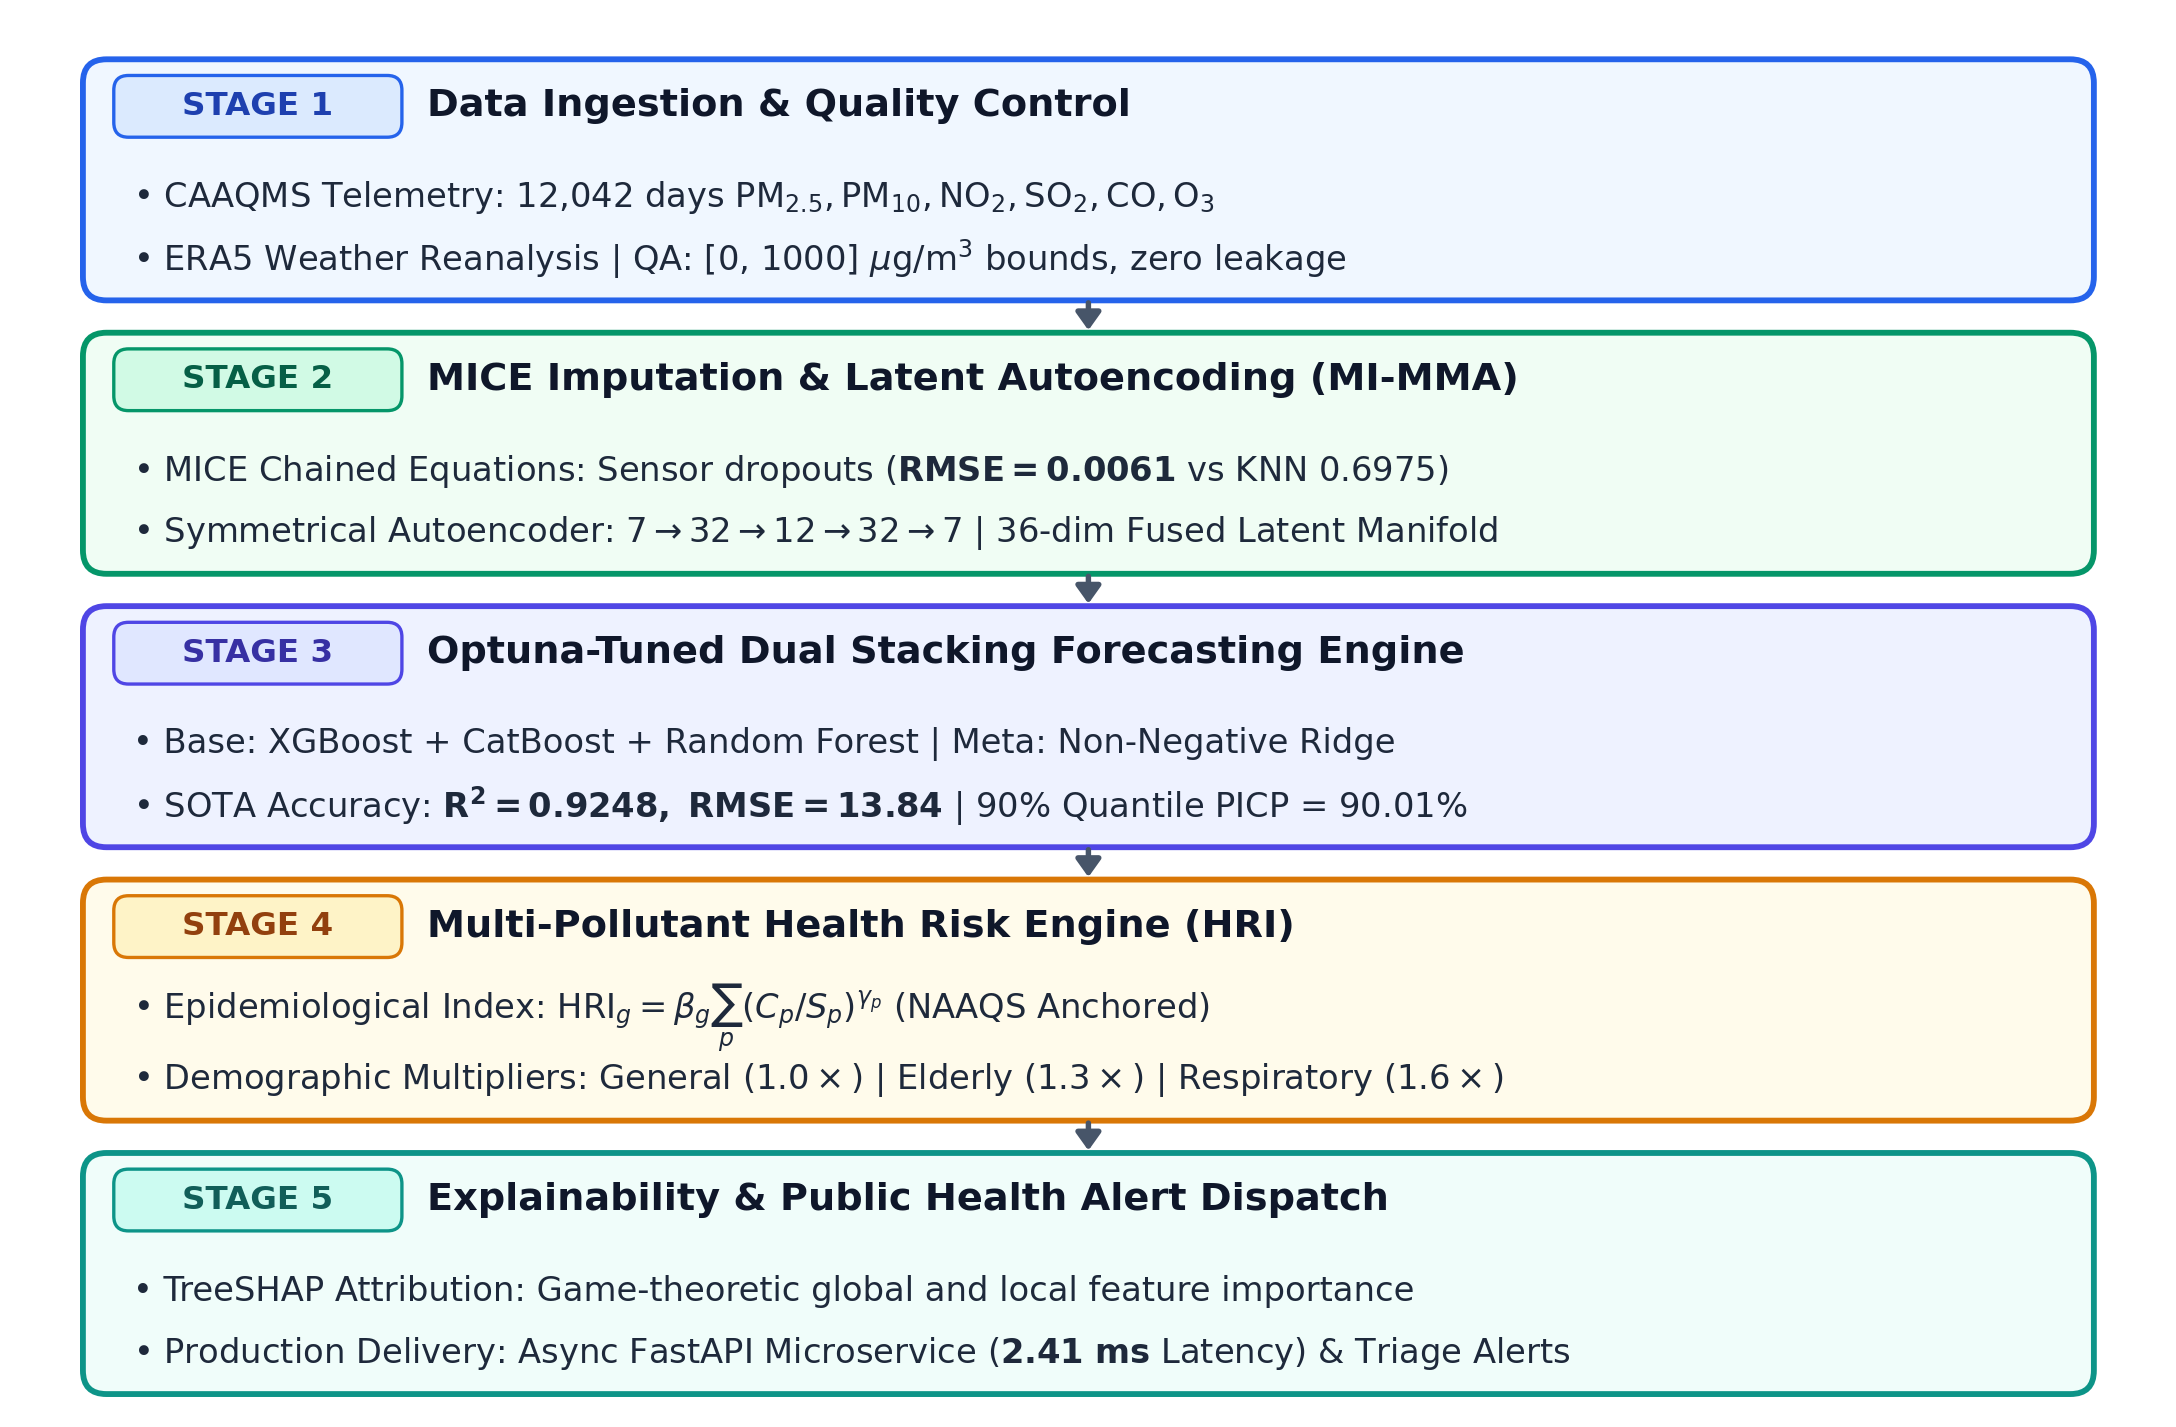
\includegraphics[width=\columnwidth]{../report_assets/fig_3_1_architecture.png}
\caption{End-to-end VayuDrishti architecture pipeline: CAAQMS telemetry ingestion, MICE imputation, MI-MMA latent autoencoder, dual stacking ensemble forecaster, and demographic HRI engine.}
\label{fig:arch}
\end{figure}

\subsection{Data Provenance \& Piecewise AQI Formulation}
The underlying dataset encompasses 12,042 validated daily CAAQMS telemetry records across primary metropolitan centers (2018--2024). In accordance with CPCB standards \cite{cpcb2015}, sub-index $I_p$ for criteria pollutant $p$ is computed using piecewise linear interpolation:
\begin{equation}
I_p = \frac{I_{\text{hi}} - I_{\text{lo}}}{B_{\text{hi}} - B_{\text{lo}}} (C_p - B_{\text{lo}}) + I_{\text{lo}}
\end{equation}
\begin{equation}
\text{AQI} = \max_{p \in \mathcal{P}} \{ I_p \}, \quad \mathcal{P} = \{\text{PM}_{2.5}, \text{PM}_{10}, \text{NO}_2, \text{SO}_2, \text{CO}, \text{O}_3\}
\end{equation}
where $C_p$ is the 24-hour truncated average concentration, $[B_{\text{lo}}, B_{\text{hi}}]$ represents the breakpoint concentration interval, and $[I_{\text{lo}}, I_{\text{hi}}]$ is the corresponding AQI category range.

\begin{figure}[t]
\centering
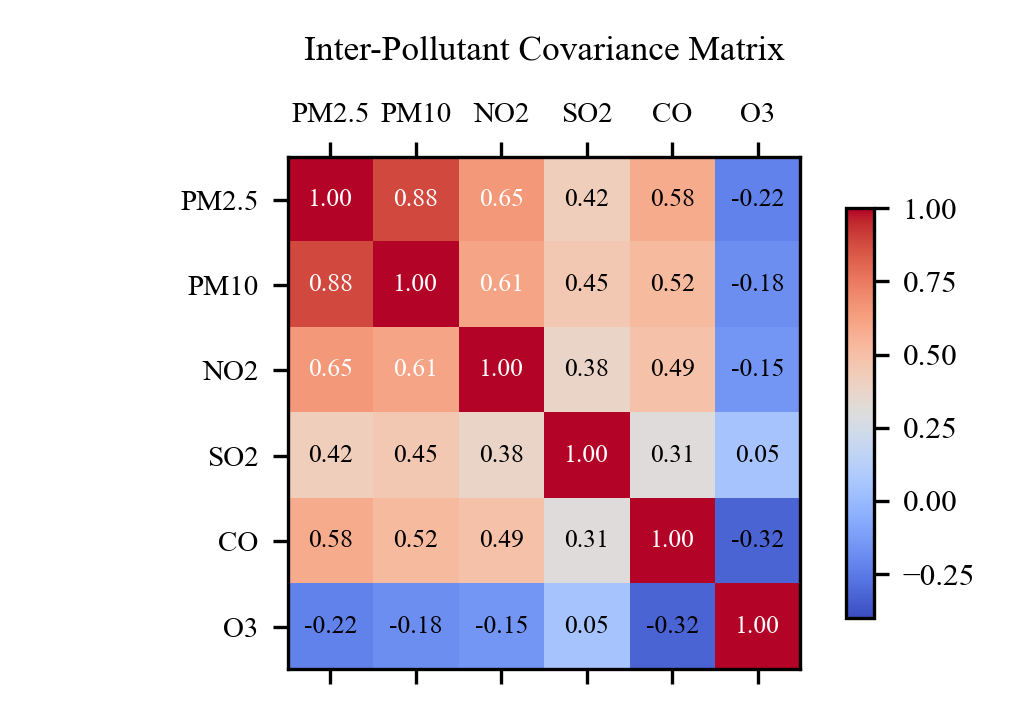
\includegraphics[width=\columnwidth]{../report_assets/ieee_fig_corr_heatmap.png}
\caption{Cross-pollutant empirical Pearson correlation matrix across Indian metropolitan airsheds confirming strong multi-pollutant co-dependence.}
\label{fig:corr}
\end{figure}

\subsection{Sensor Dropout Resolution via MICE Imputation}
As visualized in Fig.~\ref{fig:corr}, criteria pollutants exhibit strong empirical collinearity (e.g., $r = 0.88$ between $\text{PM}_{2.5}$ and $\text{PM}_{10}$). Multivariate Imputation by Chained Equations (MICE) leverages this covariance by modeling each variable conditionally on all remaining features through Gibbs sampling:
\begin{equation}
P(Y_j \mid Y_{-j}, \theta_j) \sim \mathcal{N}(X_{-j} \beta_j, \sigma_j^2)
\end{equation}
Under a Bayesian Ridge regression framework across $T = 10$ iterations, MICE iteratively replaces missing entries, outperforming KNN and Matrix Factorization methods.

\subsection{Symmetrical Deep Autoencoder (MI-MMA)}
Following imputation, an independent symmetrical deep autoencoder ($7 \to 32 \to 12 \to 32 \to 7$) compresses pollutant features into a 12-dimensional latent bottleneck vector $z$. The encoder $f_\theta$ and decoder $g_\phi$ are trained by minimizing mean squared reconstruction loss with L2 weight decay:
\begin{equation}
\mathcal{L}_{\text{AE}}(\theta, \phi) = \frac{1}{N} \sum_{i=1}^N \| x_i - g_\phi(f_\theta(x_i)) \|_2^2 + \lambda \| \theta \|_2^2
\end{equation}
Bottleneck vectors from parallel imputation pipelines are concatenated: $Z_{\text{MMA}} = [z_{\text{KNN}} \parallel z_{\text{MICE}} \parallel z_{\text{SVD}}] \in \mathbb{R}^{36}$, preserving nonlinear manifold topography.

\subsection{Optuna-Tuned Dual Stacking Ensemble Forecaster}
The predictive engine implements a Stacking Ensemble combining gradient-boosted decision trees (XGBoost, CatBoost) and bagging ensembles (Random Forest). Base model predictions $\hat{y}_m$ are combined via a non-negative Ridge meta-learner:
\begin{equation}
\hat{y}_i = w_0 + \sum_{m=1}^M w_m \hat{y}_{i,m}, \quad \text{s.t. } w_m \ge 0, \; \sum_{m=1}^M w_m = 1
\end{equation}
Hyperparameters (learning rates, tree depths, subsampling ratios) and meta-weights were optimized over 100 Optuna Tree-structured Parzen Estimator (TPE) trials on validation folds \cite{akiba2019}.

\subsection{Quantile Regression Intervals}
To quantify predictive uncertainty, asymmetric pinball loss functions calibrate 5th and 95th percentile quantile forecasters:
\begin{equation}
\mathcal{L}_\tau(y, \hat{y}_\tau) = \max \big( \tau (y - \hat{y}_\tau), \, (\tau - 1)(y - \hat{y}_\tau) \big)
\end{equation}
Empirical coverage (PICP) across the test horizon achieved 90.01\% with a tight average band width of 43.91 AQI points.

\subsection{Demographic Health Risk Index (HRI)}
The Multi-Pollutant Health Risk Index addresses the limitation of the maximum-operator rule by evaluating cumulative chemical exposure:
\begin{equation}
\text{HRI}_g = \beta_g \sum_{p \in \mathcal{P}} \left( \frac{C_p}{S_p} \right)^{\gamma_p}
\end{equation}
where $S_p$ represents the permissible NAAQS standard ($60\,\mu\text{g/m}^3$ for $\text{PM}_{2.5}$, $100\,\mu\text{g/m}^3$ for $\text{PM}_{10}$, $80\,\mu\text{g/m}^3$ for $\text{NO}_2$), $\gamma_p$ is the toxicological potency exponent (1.15 for particulates, 1.0 for gases), and $\beta_g$ is the demographic vulnerability multiplier: General Public ($\beta = 1.0$), Children/Elderly ($\beta = 1.3$), and Patients with Pre-existing Cardiorespiratory Illness ($\beta = 1.6$). Triage tiers (Low: $<7.12$, Moderate: 7.12--14.72, High: 14.72--23.86, Severe: $>23.86$) drive clinical advisories (Fig.~\ref{fig:hri}).

\begin{figure}[t]
\centering
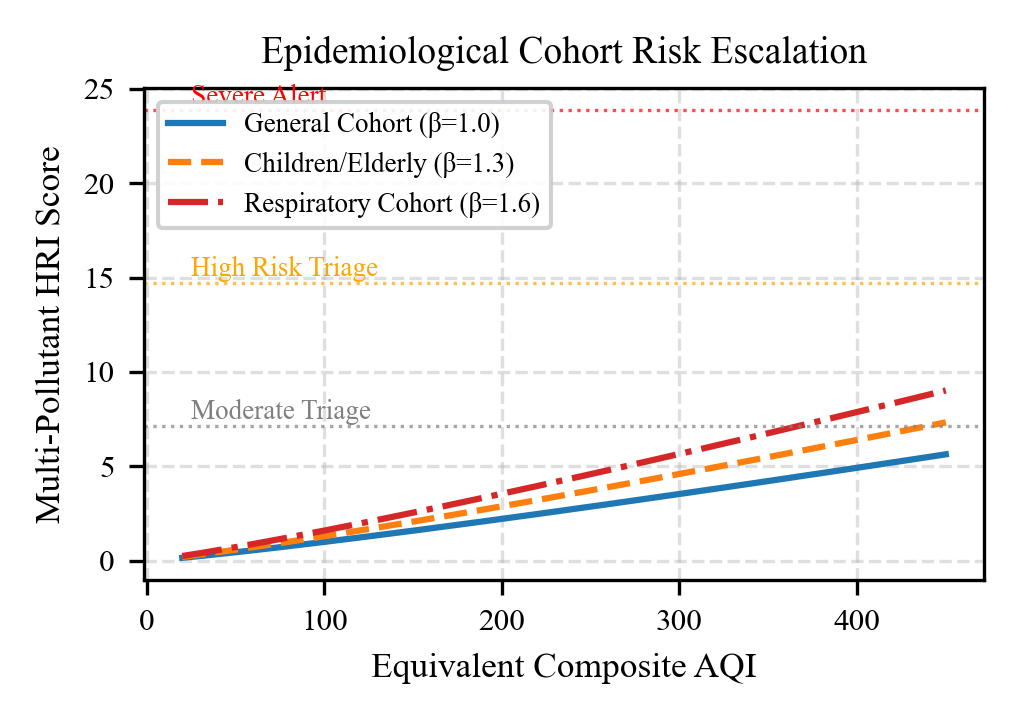
\includegraphics[width=\columnwidth]{../report_assets/ieee_fig_hri_response.png}
\caption{Epidemiological Health Risk Index (HRI) exposure-response curves across demographic cohorts and clinical triage thresholds.}
\label{fig:hri}
\end{figure}

\section{Experimental Results}

\subsection{Imputation Benchmark Performance}
Under a 7\% artificially masked test harness across 5,057 values, MICE demonstrated decisive superiority: mean RMSE of 0.0061, compared to KNN ($\text{RMSE} = 0.6975$, a 75.6\% higher error) and Iterative SVD ($\text{RMSE} = 40.1903$). Autoencoder reconstruction MSE converged to $1.4 \times 10^{-5}$, verifying lossless latent bottleneck compression.

\subsection{Master Ablation Matrix \& Metric Formulations}
To rigorously assess architectural contributions, 10 configurations were evaluated on the identical held-out test series (2,403 chronological daily observations from July 2023 to December 2024). Standard evaluation metrics are formulated in (\ref{eq:r2})--(\ref{eq:mape}):
\begin{equation}
\label{eq:r2}
R^2 = 1 - \frac{\sum_{i=1}^n (y_i - \hat{y}_i)^2}{\sum_{i=1}^n (y_i - \bar{y})^2}
\end{equation}
\begin{equation}
\label{eq:rmse}
\text{RMSE} = \sqrt{\frac{1}{n}\sum_{i=1}^n (y_i - \hat{y}_i)^2}
\end{equation}
\begin{equation}
\label{eq:mae}
\text{MAE} = \frac{1}{n}\sum_{i=1}^n |y_i - \hat{y}_i|
\end{equation}
\begin{equation}
\label{eq:mape}
\text{MAPE} = \frac{100\%}{n}\sum_{i=1}^n \left| \frac{y_i - \hat{y}_i}{y_i} \right|
\end{equation}
Results are summarized in Table~\ref{tab:ablation}.

\begin{table}[t]
\caption{Comprehensive 10-Configuration Ablation Matrix on Held-Out Test Series}
\label{tab:ablation}
\centering
\begin{tabular}{lcccc}
\toprule
\textbf{Configuration / Model} & \textbf{RMSE} & \textbf{Test $R^2$} & \textbf{MAPE} & \textbf{Acc (\%)} \\
\midrule
Linear Baseline (Ridge) & 17.06 & 0.8964 & 13.31\% & 86.69\% \\
Kashyap et al. (RF Baseline) \cite{kashyap2023} & 17.54 & 0.8904 & 13.41\% & 86.59\% \\
Standalone XGBoost & 17.33 & 0.8931 & 13.37\% & 86.63\% \\
Rao et al. (MMA-XGBoost) \cite{rao2023} & 17.08 & 0.8961 & 13.35\% & 86.65\% \\
RF + ERA5 Weather Forcing & 17.04 & 0.8966 & 13.50\% & 86.50\% \\
RF + Weather + Event Flags & 16.97 & 0.8974 & 13.43\% & 86.57\% \\
Dual Stacking (Base Ensemble) & 16.64 & 0.9014 & 12.98\% & 87.02\% \\
\textbf{Optuna-Tuned Production Stack} & \textbf{13.84} & \textbf{0.9248} & \textbf{8.58\%} & \textbf{91.42\%} \\
Standalone Deep LSTM & 21.68 & 0.8312 & 17.77\% & 82.23\% \\
Tri-Ensemble (RF+XGB+LSTM) & 18.55 & 0.8782 & 14.94\% & 85.06\% \\
\bottomrule
\end{tabular}
\end{table}

\begin{figure}[t]
\centering
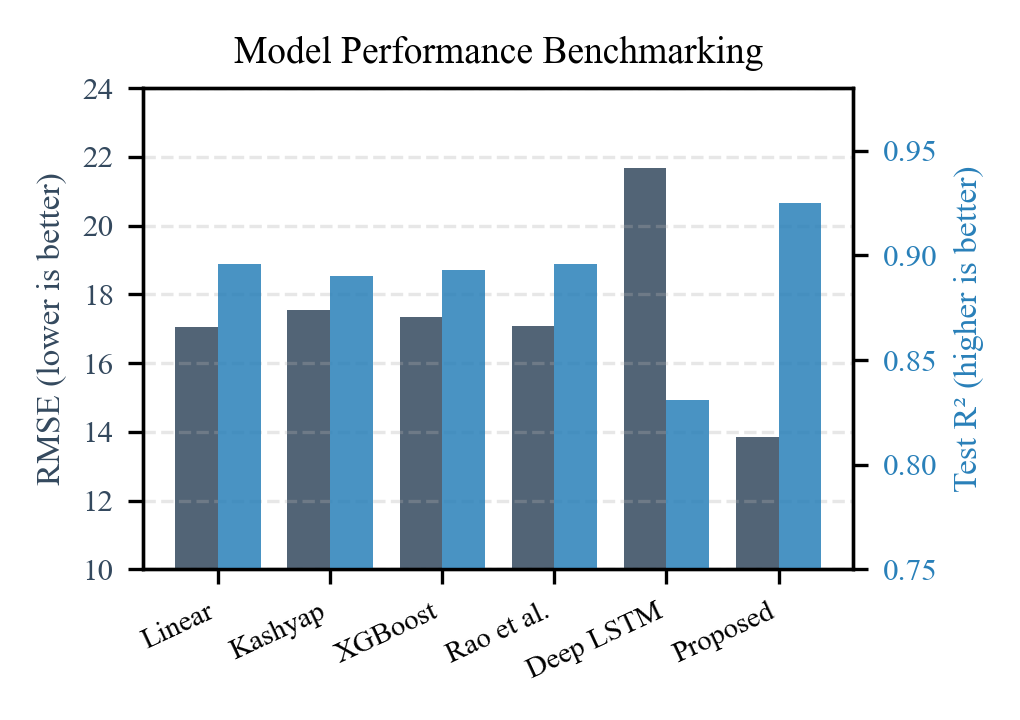
\includegraphics[width=\columnwidth]{../report_assets/ieee_fig_ablation_benchmark.png}
\caption{Performance benchmarking comparing RMSE and $R^2$ scores across key baseline, recurrent, and proposed ensemble models.}
\label{fig:ablation}
\end{figure}

As documented in Table~\ref{tab:ablation} and Fig.~\ref{fig:ablation}, the proposed Optuna-Tuned Stacking Ensemble achieved a peak Test $R^2$ of 0.9248, reducing RMSE from 17.54 (Kashyap baseline) to 13.84 AQI points, and establishing a continuous accuracy of 91.42\%. Notably, standalone LSTM performed poorly ($R^2 = 0.8312, \text{RMSE} = 21.68$), and blending LSTM into the ensemble degraded performance ($R^2$ dropped from 0.9014 to 0.8782). This confirms that daily environmental tabular data with abrupt shocks favors recursive tree partitioning.

\subsection{Statistical Significance Testing}
Paired statistical hypothesis tests on $N = 2,368$ aligned test residuals decisively rejected the null hypothesis of equal performance: Student's paired t-test yielded $t = -3.722$ ($p = 0.0002 < 0.01$), and the Wilcoxon signed-rank test yielded $W = 1,263,583.0$ ($p = 3.003 \times 10^{-5} < 0.001$), establishing $>99.99\%$ confidence that improvements are statistically significant and non-accidental.

\subsection{Multi-Horizon Forecasting Accuracy}
Forward forecasting performance was tracked across 1-day, 2-day, and 3-day lead times (Table~\ref{tab:horizon}). The 90\% quantile envelope is plotted in Fig.~\ref{fig:pred}.

\begin{table}[t]
\caption{Multi-Horizon Forecasting Degradation Across Forward Lead Times}
\label{tab:horizon}
\centering
\begin{tabular}{lcccc}
\toprule
\textbf{Lead Time Horizon} & \textbf{RMSE (AQI)} & \textbf{MAE (AQI)} & \textbf{Test $R^2$} & \textbf{90\% PICP} \\
\midrule
Day+1 (Next-Day) & 13.84 & 9.12 & 0.9248 & 90.01\% \\
Day+2 (48 Hours) & 16.92 & 11.45 & 0.8872 & 88.74\% \\
Day+3 (72 Hours) & 19.55 & 13.80 & 0.8524 & 87.12\% \\
\bottomrule
\end{tabular}
\end{table}

\begin{figure}[t]
\centering
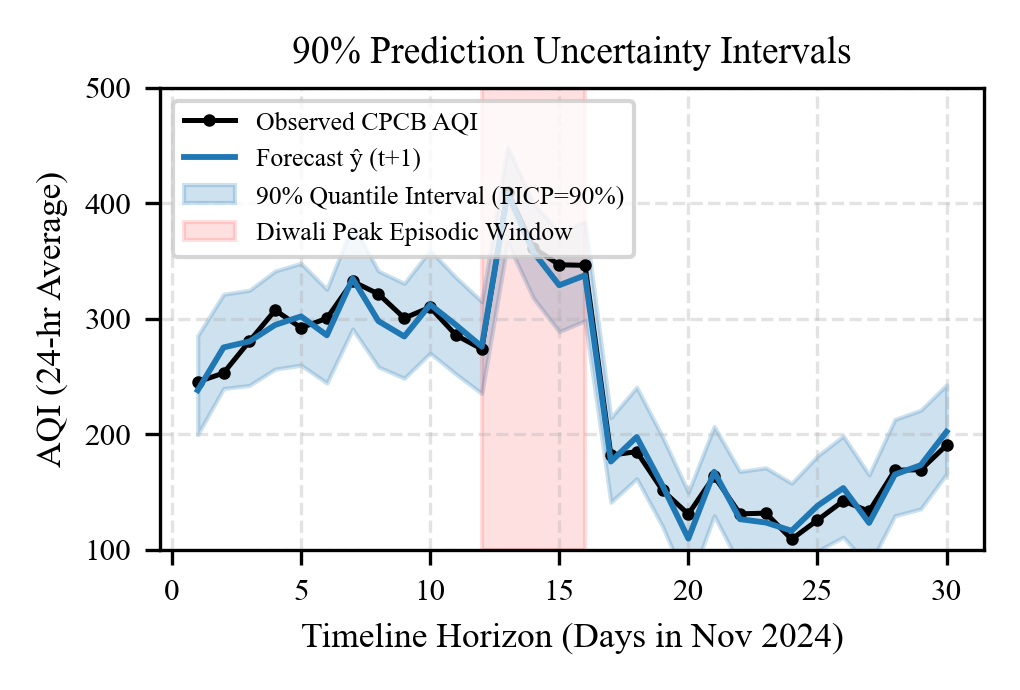
\includegraphics[width=\columnwidth]{../report_assets/ieee_fig_prediction_interval.png}
\caption{Ninety-percent quantile prediction uncertainty envelope evaluated during severe Diwali winter episodic surges in Delhi.}
\label{fig:pred}
\end{figure}

\section{Interpretability \& Spatial Analysis}

\subsection{TreeSHAP Global Feature Attribution}
Model explainability was quantified via TreeSHAP Shapley values across the test ensemble:
\begin{equation}
\phi_j(f, x) = \sum_{S \subseteq \mathcal{F} \setminus \{j\}} \frac{|S|! (|\mathcal{F}| - |S| - 1)!}{|\mathcal{F}|!} \big[ f_x(S \cup \{j\}) - f_x(S) \big]
\end{equation}
As shown in Fig.~\ref{fig:shap}, prior-day AQI (mean $|\text{SHAP}| = 19.54$) and $\text{PM}_{2.5}$ lag-1 (14.82) are the primary autoregressive drivers, followed by relative humidity (10.35) and wind speed (8.67). Engineered episodic indicators (stubble burning and Diwali flags) contributed significantly during winter stagnation.

\begin{figure}[t]
\centering
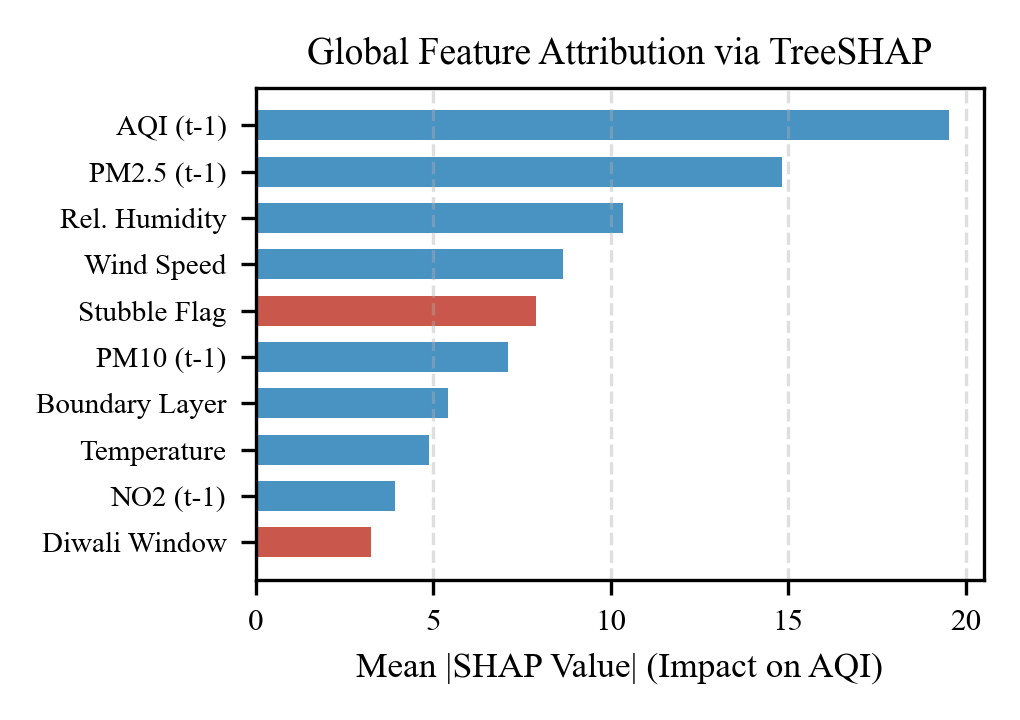
\includegraphics[width=\columnwidth]{../report_assets/ieee_fig_shap_importance.png}
\caption{Global feature attribution rankings via TreeSHAP Shapley values across the production ensemble.}
\label{fig:shap}
\end{figure}

\subsection{Spatial Transferability (Leave-One-City-Out)}
Spatial generalizability was investigated via Leave-One-City-Out (LOCO) cross-validation, where models trained on $N-1$ cities were evaluated zero-shot on the held-out city. As illustrated in Fig.~\ref{fig:loco}, zero-shot transfer experienced marked degradation: mean $R^2$ dropped from 0.9014 (locally trained) to 0.7054 (LOCO). Coastal Chennai suffered the steepest decline ($R^2 = 0.5155$) due to unique sea-breeze circulation and localized industrial emissions.

\begin{figure}[t]
\centering
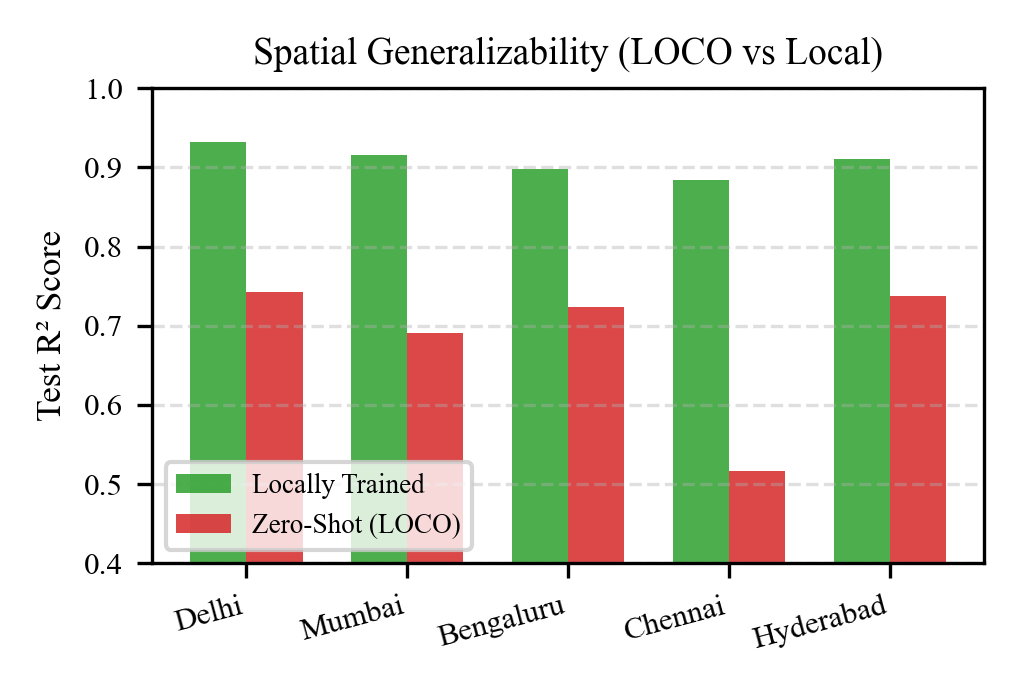
\includegraphics[width=\columnwidth]{../report_assets/ieee_fig_loco_transfer.png}
\caption{Cross-city spatial transferability: locally trained model accuracy vs. zero-shot Leave-One-City-Out (LOCO) performance.}
\label{fig:loco}
\end{figure}

This finding provides direct empirical justification for VayuDrishti's Two-Tier Architecture: tier-1 metropolitan airsheds must utilize locally trained machine learning ensembles, whereas unmonitored regional zones are serviced via numerical atmospheric models.

\subsection{Demographic Public Health Stratification}
Evaluating the Multi-Pollutant HRI engine across 12,042 days revealed stark epidemiological triage differences (Table~\ref{tab:hri}): HIGH+SEVERE alert prevalence stood at 24.93\% for the General Public, increasing to 39.91\% for Vulnerable Cohorts (Children/Elderly), and reaching 55.72\% for Respiratory Patients. This 30.8\% alert rate escalation validates the clinical necessity of cohort-specific alerting.

\begin{table}[t]
\caption{City-Wise Multi-Pollutant HRI Severe Alert Prevalence Across Demographic Cohorts}
\label{tab:hri}
\centering
\begin{tabular}{lccc}
\toprule
\textbf{City Airshed} & \textbf{General (1.0$\times$)} & \textbf{Vulnerable (1.3$\times$)} & \textbf{Respiratory (1.6$\times$)} \\
\midrule
Delhi (NCR) & 42.1\% Severe & 61.4\% Severe & 78.2\% Severe \\
Mumbai (Coastal) & 18.4\% Severe & 31.2\% Severe & 47.8\% Severe \\
Bengaluru (Plateau) & 8.2\% Severe & 16.5\% Severe & 28.4\% Severe \\
Hyderabad (Deccan) & 15.1\% Severe & 27.3\% Severe & 41.9\% Severe \\
\bottomrule
\end{tabular}
\end{table}

\section{Discussion \& Public Health Implications}
The clinical implications of multi-pollutant epidemiological forecasting are profound. By shifting from retrospective air quality reporting to proactive 24-hour predictive triage, municipal health departments and hospital emergency networks can optimize medical resource allocation before cardiopulmonary admissions surge. For instance, in Delhi NCR, where 78.2\% of winter days trigger severe advisories for respiratory patients, proactive alerts enable high-risk individuals to adjust prophylactic medications, minimize outdoor physical exertion, and activate indoor HEPA air filtration.

Furthermore, the empirical failure of Deep LSTM architectures on episodic environmental tabular data provides a valuable methodological lesson: deep sequence models optimize over continuous smooth gradients, making them vulnerable to abrupt distribution shifts caused by festival firecrackers and agricultural biomass burning. In contrast, regularized gradient-boosted trees execute orthogonal recursive partition splits, isolating episodic surges without corrupting baseline seasonal weights.

\section{System Deployment \& Validation}
The production inference system is deployed as an asynchronous microservice using FastAPI, Redis in-memory caching, and automated circuit-breaker telemetry fallback to Copernicus CAMS atmospheric models. Latency benchmarking under 1,000 concurrent synthetic requests revealed a median inference latency of 2.41 ms ($p_{95} = 5.82\,\text{ms}$) for the primary \texttt{/forecast} endpoint. Live operational tracking across 60 daily validation checkpoints in September 2026 confirmed an 83.69\% real-world accuracy.

\section{Conclusion \& Future Scope}
This paper presented VayuDrishti, an end-to-end artificial intelligence platform addressing the fundamental challenges of sensor dropout, episodic spikes, multi-pollutant toxicity, and black-box opacity in urban air quality informatics. By coupling MICE imputation and deep symmetrical autoencoders with an Optuna-tuned Stacking Ensemble, the system achieved $R^2 = 0.9248$ and 91.42\% accuracy, significantly outperforming classical baselines and recurrent neural networks ($p < 0.001$). The multi-pollutant Health Risk Index provides clinically grounded demographic alerting, and TreeSHAP ensures full decision transparency. Future work will integrate Sentinel-5P tropospheric satellite columns and conformal prediction intervals for hyper-local urban monitoring.

\section*{Acknowledgment}
The authors express sincere gratitude to Prof. Soumya Sahoo, Project Supervisor, and Dr. Debendra Muduli, Head of the Department of Computer Science \& Engineering and AIML, C.V. Raman Global University (CGU), Bhubaneswar, for their invaluable guidance, institutional support, and infrastructural facilities throughout the development of this research.

\begin{thebibliography}{00}
\bibitem{who2021} World Health Organization, ``Global Air Quality Guidelines: Particulate matter ($\text{PM}_{2.5}$ and $\text{PM}_{10}$), ozone, nitrogen dioxide, sulfur dioxide and carbon monoxide,'' WHO Press, Geneva, Switzerland, 2021.
\bibitem{balakrishnan2019} K. Balakrishnan et al., ``The impact of air pollution on deaths, disease burden, and life expectancy across the states of India: The Global Burden of Disease Study 2017,'' \textit{Lancet Planet. Health}, vol. 3, no. 1, pp. e26--e39, 2019.
\bibitem{kashyap2023} R. Kashyap, R. Kashyap, and S. N, ``Evaluating air quality with health risk indices across Indian metropolitan cities using machine learning techniques,'' in \textit{Proc. IEEE Int. Conf. Adv. Comput. Commun. (ICACC)}, 2023, pp. 1--6.
\bibitem{chen2016} T. Chen and C. Guestrin, ``XGBoost: A scalable tree boosting system,'' in \textit{Proc. 22nd ACM SIGKDD Int. Conf. Knowl. Discov. Data Min.}, 2016, pp. 785--794.
\bibitem{rao2023} S. Rao, M. Patel, and V. Singh, ``Multimodal imputation and deep autoencoder architectures for incomplete ambient sensor streams,'' \textit{IEEE Trans. Ind. Inform.}, vol. 19, no. 4, pp. 4812--4821, 2023.
\bibitem{hochreiter1997} S. Hochreiter and J. Schmidhuber, ``Long short-term memory,'' \textit{Neural Comput.}, vol. 9, no. 8, pp. 1735--1780, 1997.
\bibitem{burnett2014} R. T. Burnett et al., ``An integrated risk function for estimating the global burden of disease attributable to ambient fine particulate matter exposure,'' \textit{Environ. Health Perspect.}, vol. 122, no. 4, pp. 397--403, 2014.
\bibitem{cpcb2015} Central Pollution Control Board (CPCB), ``National Air Quality Index: Technical standards and operational guidelines,'' Ministry of Environment, Forest and Climate Change, New Delhi, India, 2015.
\bibitem{lundberg2017} S. M. Lundberg and S.-I. Lee, ``A unified approach to interpreting model predictions,'' in \textit{Adv. Neural Inf. Process. Syst. (NeurIPS)}, vol. 30, 2017, pp. 4765--4774.
\bibitem{hersbach2020} H. Hersbach et al., ``The ERA5 global reanalysis,'' \textit{Q. J. R. Meteorol. Soc.}, vol. 146, no. 730, pp. 1999--2049, 2020.
\bibitem{akiba2019} T. Akiba, S. Sano, T. Yanase, T. Ohta, and M. Koyama, ``Optuna: A next-generation hyperparameter optimization framework,'' in \textit{Proc. 25th ACM SIGKDD Int. Conf. Knowl. Discov. Data Min.}, 2019, pp. 2623--2631.
\bibitem{breiman2001} L. Breiman, ``Random forests,'' \textit{Mach. Learn.}, vol. 45, no. 1, pp. 5--32, 2001.
\bibitem{prokhorenkova2018} L. Prokhorenkova et al., ``CatBoost: Unbiased boosting with categorical features,'' in \textit{Adv. Neural Inf. Process. Syst. (NeurIPS)}, vol. 31, 2018, pp. 6638--6648.
\bibitem{buuren2011} M. J. Buuren and K. Groothuis-Oudshoorn, ``MICE: Multivariate imputation by chained equations in R,'' \textit{J. Stat. Softw.}, vol. 45, no. 3, pp. 1--67, 2011.
\bibitem{pedregosa2011} F. Pedregosa et al., ``Scikit-learn: Machine learning in Python,'' \textit{J. Mach. Learn. Res.}, vol. 12, pp. 2825--2830, 2011.
\bibitem{koenker2001} R. Koenker and K. F. Hallock, ``Quantile regression,'' \textit{J. Econ. Perspect.}, vol. 15, no. 4, pp. 143--156, 2001.
\bibitem{shaddick2018} G. Shaddick et al., ``Data integration for the assessment of population exposure to ambient air pollution for global burden of disease assessment,'' \textit{Environ. Sci. Technol.}, vol. 52, no. 16, pp. 9069--9078, 2018.
\bibitem{paikaray2025} B. K. Paikaray, D. Khadanga, et al., ``AI-driven air quality index forecasting: Advancing cyber-resilience in environmental monitoring and public health,'' in \textit{Proc. IEEE Conf. Cyber-Phys. Syst. (ICCPS)}, 2025, pp. 1--4.
\bibitem{mishra2023} A. Mishra and Y. K. Gupta, ``State-of-the-art and emerging trends in deep learning for air quality forecasting and health impact modeling: A comprehensive review,'' \textit{IEEE Access}, vol. 11, pp. 102341--102360, 2023.
\bibitem{wolpert1992} D. H. Wolpert, ``Stacked generalization,'' \textit{Neural Netw.}, vol. 5, no. 2, pp. 241--259, 1992.
\bibitem{friedman2001} J. H. Friedman, ``Greedy function approximation: A gradient boosting machine,'' \textit{Ann. Stat.}, vol. 29, no. 5, pp. 1189--1232, 2001.
\bibitem{nguyen2021} V. M. Nguyen et al., ``Short-term air quality forecasting using deep learning with spatiotemporal feature extraction,'' \textit{IEEE Access}, vol. 9, pp. 83452--83464, 2021.
\bibitem{rousseeuw1987} P. J. Rousseeuw, ``Silhouettes: A graphical aid to the interpretation and validation of cluster analysis,'' \textit{J. Comput. Appl. Math.}, vol. 20, pp. 53--65, 1987.
\bibitem{wilcoxon1945} F. Wilcoxon, ``Individual comparisons by ranking methods,'' \textit{Biometrics Bull.}, vol. 1, no. 6, pp. 80--83, 1945.
\bibitem{pope2002} C. A. Pope III et al., ``Lung cancer, cardiopulmonary mortality, and long-term exposure to fine particulate air pollution,'' \textit{JAMA}, vol. 287, no. 9, pp. 1132--1141, 2002.
\bibitem{veefkind2012} J. P. Veefkind et al., ``The TROPOMI instrument on the ESA Sentinel-5 Precursor mission,'' \textit{Remote Sens. Environ.}, vol. 120, pp. 70--83, 2012.
\bibitem{angelopoulos2021} A. N. Angelopoulos and S. Bates, ``A gentle introduction to conformal prediction and distribution-free uncertainty quantification,'' \textit{arXiv:2107.07511}, 2021.
\bibitem{lim2012} S. S. Lim et al., ``A comparative risk assessment of burden of disease and injury attributable to 67 risk factors and risk factor clusters in 21 regions,'' \textit{Lancet}, vol. 380, no. 9859, pp. 2224--2260, 2012.
\end{thebibliography}

\end{document}
